\documentclass[12pt]{article}
\usepackage[top=0.8in, bottom=1in, left=1.1in, right=1.1in]{geometry} 
\usepackage[all]{xy}
\usepackage{setspace}
\usepackage{float}
\usepackage{algorithm}
\usepackage{algcompatible}
\usepackage{enumitem}
%\usepackage{biblatex}
\author{
  Souleyman Boudouh, Clément Charmillot, Emilien Guandalino\\
}



\usepackage{amsmath,amsthm,amssymb,color,latexsym}
\usepackage{geometry}        
\geometry{letterpaper}    
\usepackage{graphicx}


\begin{document}

\title{CS-471 Stage 2 Project report}
\date{}
\maketitle

\vspace{-3em}

\section{Recall from last time}

We shortly remind here the previous status of the project at the end of the stage 1 report.

\vspace{0.5em}

\noindent \textit{Problem:} We are trying to create a load-aware load generator which can maximize the load/throughput for a given workload within a tail latency constraint.

\vspace{0.5em}

\noindent \textit{Hypothesis:} When increasing the load, the increase in latency can either be inherent to the given workload, ie \textit{inherent latency}, or simply caused by the change itself, ie \textit{transient latency}. We expect the transient latency to settle down after some time.

\vspace{0.5em}

\noindent \textit{Solution:} Factor analysis, ie model the latency as a function of throughput and different factors which we manually classify as either inherent or transient. Maximum is reached when inherent latency reaches tail latency constraint.

\section{Updated Research Problem}

\textit{Hypothesis:} We continue our attempt to solve this problem by maintaining the same hypothesis, which we believe to be true. However we have completely changed our proposed solution and abandoned the factor analysis. Here are a few reasons why we have decided to change:

\begin{enumerate}
	\item Factor analysis is a much harder problem than what is necessary for our purpose. It requires understanding exactly from where the latency is coming from, proper modeling and precise measurement of each factor during execution. This is an entirely new research problem, and although interesting, it is beyond the scope of our project.
	\item  It requires the researcher to implement measurement and adaptation of all factors for each new workload which we are testing. This is a lot of work, which defeats the initial purpose of simplifying the testing process.
	\item We can achieve the same result with a simpler approach, which detail below.
\end{enumerate}

\noindent \textit{New Solution:} Based on our stated hypothesis, we already assume that the variance goes through a transient phase until it eventually converges to its inherent value. We can therefore detect the point at which the transient latency has settled down by experimentally looking at the convergence rate of the latency. Figure 1 shows what this behavior would look like, and we expect to find similar effects in latency measurements. 

\clearpage
\begin{figure}[H]
  \centering
  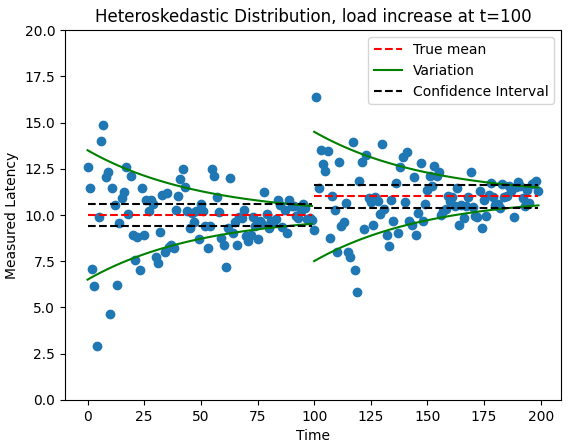
\includegraphics[width=0.6\textwidth]{distrib.png}
  \caption{Hypothetic Latency Distribution}
  \label{fig:sample}
\end{figure}

\noindent We can see on the graph that with time, variance decreases as transient latency settles down. At time $t=100$, we have reached our confidence interval, at which point we decide that it is safe to increase the workload. This change causes the variance to increase again, before settling down to a new maximum. We iterate through this process, until we have good statistical certainty that we have reached maximum throughput within a tail latency constraint. 

\noindent Compared to factor analysis, this strategy only requires us to experimentally measure latency from our system which we treat as a black box. This however raises some new theoretical questions which we explain in the next section.

\singlespacing

\noindent \textit{Related Work:} As explained in the Stage 1 report, and after further investigation, we find a large amount of literature around tail latency, its characterization and its sources. Once again, our purpose is different from those papers since we are in a testing environment in which we have control over the system load, unlike in production.


\section{Questions, Hypotheses and Test}

In this section, we discuss the new theoretical questions which are raised by our new approach. In the next section, we will give more information as to where each of those questions fit into the global picture.
\singlespacing


\noindent \textit{Questions:} Here are the new theoretical issues which we are currently working on: 

\begin{enumerate}
	\item \textit{Sampling Interval}: When evaluating a workload, we perform a set number of operations over which we then measure latency for this period. However, there are no simple solutions to determine how long this sampling period should be in order to guarantee that our measurement is accurate enough. There are multiple parameters which we should take into account to determine this window:
		\begin{enumerate}
			\item Accuracy \& Confidence Intervals: How accurately do we want to estimate latency? How much certainty do we want about our measure ? More accuracy and certainty imply larger sampling windows.
			\item Variability: How variable is the metric that we are observing ? Greater variability implies more samples for accurate estimation.
			\item Effect Size: How large is the effect size that we are measuring ? Accurately measuring small changes require more samples.
			\item Time Homogeneity: How to correctly sample a distribution which changes over time ? This will affect the different sampling windows that we consider for measurement.
		\end{enumerate}

		We are still looking into different statistical tools, such as Power Analysis, which enable us determine sampling size when considering all those factors. Since we still have not yet figured out a full solution, we have used a fixed sampling window size when performing our measurements.

	\item \textit{Convergence Detection}: There are two levels at which we need to detect convergence:
		\begin{enumerate}[label=2.\arabic*.]
			\item At each iteration: When do we decide that we have converged to inherent latency? If we are above the tail latency requirement we may have to decrease load again, but we must first be sure that we have actually converged.
			\item Across iterations: When do we decide that we have found a global maximum and output a result ? We may oscillate around the optimum for many iterations.
		\end{enumerate}

	\item \textit{Workload Increase Step Size}: When we decide to increase workload, by how much should we increase it ?

	\item \textit{Hysteresis}: When evaluating complex systems, even with proper methodology and the correct amount of samples, two different runs might converge to different values. This is a difficult problem to address, and we will first try to optimize for a single run, before trying to optimize across runs.
\end{enumerate}

\noindent \textit{Testing:} Concerning the test of our hypothesis, we will give more details in the following section. For the theoretical issues mentioned above, we first need to ensure that our mathematical derivations are rigorous, then we need test our code implementations and finally we can run the workloads and experimentally tune the parameters, ex: confidence interval size, for best results. As a reference, we can compare the output of our solution with the results given in the Tailbench paper.

\section{Progress, Result and Analysis}

\textit{Experimental Setup}: In order to test our hypothesis, we used the code provided by the Tailbench testing suite. For reasons detailed in the "Challenges" section, we decided to use Silo, an OLTP database, with a TPC-C benchmark. We ran our experiment in integrated configuration, i.e. all operations happen in memory (no disk, no network access), with a single thread and a single warehouse.

\singlespacing
\noindent \textit{Hypothesis test}:
\noindent Here are the results that we obtained:

\begin{figure}[H]
  \centering
  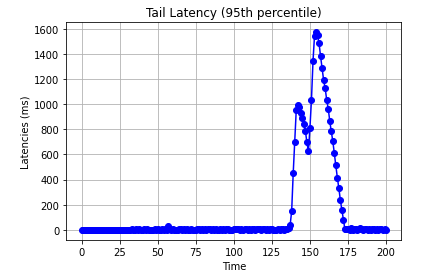
\includegraphics[width=0.6\textwidth]{95percent.png}
  \caption{Tail Latency Measurement}
  \label{fig:sample}
\end{figure}

\noindent As we can see, the tail latency greatly increases when we perform a change in workload, and eventually converges back to its inherent state. Now that we have a good reason to believe that our hypothesis is correct, we propose an algorithm which exploits this hypothesis in order to solve our problem.

\vspace{0.5em}
\noindent \textit{Algorithm Design}: Here is the algorithm, the numbers on the right indicate to which theoretical problem each method corresponds to.

\begin{algorithm}
	\caption{Load-Aware Load Generator}\label{alg:cap}
	\begin{algorithmic}[1]
		\STATE Initialize workload data structures
		\STATE running $\gets$ true
		\WHILE{running}
		\STATE num\_requests $\gets$ find\_sampling\_window() \hfill Problem 1.
		\STATE run\_workload(num\_requests)
		\STATE latency $\gets$ aggregate\_latencies()
		\STATE converged $\gets$ latency\_convergence(latency, confidence\_interval) \hfill Problem 2.1
		\IF{converged}
		\IF{ global\_convergence(latency, latency\_requirement)} \hfill Problem 2.2
		\STATE \textbf{return} (load, latency) 
		\ELSIF{latency $<$ latency\_requirement}
		\STATE increase\_load() \hfill Problem 3.
		\ELSIF{latency $>$ latency\_requirement}
		\STATE decrease\_load()\hfill Problem 3.
		\ENDIF
		\ENDIF
		\ENDWHILE
	\end{algorithmic}
\end{algorithm}

\noindent In our current implementation, we have simplified each sub-problem in order to be able to make first measurements for our hypothesis test. Improving this algorithm will be the next focus of our project.

\singlespacing


\section{Challenges}

We encountered many unexpected practical challenges when trying to verify our hypothesis. The first one is working with the Tailbench repository code. The Tailbench suite uses Harness, a tail latency measurement software, to run multiple different benchmarks which have been adapted for this purpose. Both the Harness code and the benchmarks have not been maintained for years, and come with multiple dependency problems, various compilation errors and segmentation faults which we had to debug with GDB.  Understanding and making changes to such a large codebase was tedious and time-consuming.

\singlespacing

\noindent Another challenge that we had was to adapt the way Tailbench performs latency measurements. Tailbench is designed to aggregate statistics about latencies during execution and then dump them into a binary file which we have to parse with a python script afterwards. This is unsuitable for our purpose, since we have to take decisions based on the latency during the execution. If we are not able to modify the workload and observe latency in live, then all of our analysis falls apart. We therefore had to modify the code in order to continuously iterate over a given workload and collect the associated latencies.

\section{Plan}

We do not have any team member changes. In terms of priority, now that we have verified our hypothesis, we can move on to the next step which means: finishing our algorithm implementation, experimenting with different solutions for the theoretical problems, and evaluating them on our benchmark. Our schedule now reflects those objectives.

\section{TLDR}

\textit{Research}: We have not changed our goal or hypothesis. We have changed our approach. Now we treat our system as a blackbox and only measure latency.

\singlespacing
\noindent \textit{Progress}: We have tested our initial hypothesis, it works. We have implemented a simple algorithm based on that. A few theoretical questions remain to improve the algorithm.

\singlespacing
\noindent \textit{Next steps}: Implement different solutions to the problem, evaluate them.


%\bibliographystyle{IEEEtran}
%\bibliography{ref}

\end{document}
